\section*{Problem 10}
\begin{proof} [Solution]
	Follow the algorithm:
	\begin{enumerate} [Step 1]
		\item Create adjacency matrix $M$ for the given graph. 
		\item Replace all the diagonals of $M$ with the degree of nodes. For example, if $\deg(1)=3$, then put $m_{1,1}=3$ which is an element of $M$.
		\item Replace all non-diagonal 1’s with -1.
		\item Remove any one row and one column of $M$. Let the remained be $M^*$.
		\item Calculate $\det M^*$. This is the total number of spanning trees. Done!
	\end{enumerate}
	Note that Step 4 and Step 5 are the same as calculate co-factor for any element of $M$. Co-factor for all the elements will be same. Now, let the graph be
	\begin{center}
		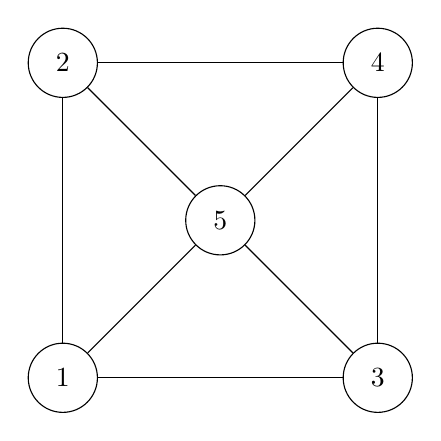
\begin{tikzpicture}
			\tikzstyle{Vertex} = [circle, draw, minimum size=25, inner sep=0pt]	
			\node (1) at (0,0) [Vertex, fill=white] {1};
			\node (2) at (0,4) [Vertex, fill=white] {2};
			\node (3) at (4,0) [Vertex, fill=white] {3};
			\node (4) at (4,4) [Vertex, fill=white] {4};
			\node (5) at (2,2) [Vertex, fill=white] {5};
			\draw [-] (1) to (2);
			\draw [-] (1) to (3);
			\draw [-] (1) to (5);
			\draw [-] (2) to (4);
			\draw [-] (2) to (5);
			\draw [-] (3) to (5);
			\draw [-] (3) to (4);
			\draw [-] (4) to (5);
		\end{tikzpicture}
	\end{center}
	For the graph, the adjacency matrix is
	\begin{center}
		\begin{equation*}
			M = \begin{pmatrix} 
				0 & 1 & 1 & 0 & 1 \\
				1 & 0 & 0 & 1 & 1 \\
				1 & 0 & 0 & 1 & 1 \\
				0 & 1 & 1 & 0 & 1 \\
				1 & 1 & 1 & 1 & 0
			\end{pmatrix} 
		\end{equation*}
	\end{center}
	Replace all the diagonals of $M$ with the degree of nodes.
	\begin{center}
		\begin{equation*}
			M = \begin{pmatrix} 
				{\color{red}3} & 1 & 1 & 0 & 1 \\
				1 & {\color{red}3} & 0 & 1 & 1 \\
				1 & 0 & {\color{red}3} & 1 & 1 \\
				0 & 1 & 1 & {\color{red}3} & 1 \\
				1 & 1 & 1 & 1 & {\color{red}4}
			\end{pmatrix} 
		\end{equation*}
	\end{center}
	Replace all non-diagonal 1’s with -1.
	\begin{center}
		\begin{equation*}
			M = \begin{pmatrix} 
				3 & {\color{red}-1} & {\color{red}-1} & 0 & {\color{red}-1} \\
				{\color{red}-1} & 3 & 0 & {\color{red}-1} & {\color{red}-1} \\
				{\color{red}-1} & 0 & 3 & {\color{red}-1} & {\color{red}-1} \\
				0 & {\color{red}-1} & {\color{red}-1} & 3 & {\color{red}-1} \\
				{\color{red}-1} & {\color{red}-1} & {\color{red}-1} & {\color{red}-1} & 4
			\end{pmatrix} 
		\end{equation*}
	\end{center}
	Remove any one row and one column of $M$. I choose the last row and last column. Let the remained be $M^*$.
	\begin{center}
		\begin{equation*}
			M^* = \begin{pmatrix} 
				3 & -1 & -1 & 0 \\
				-1 & 3 & 0 & -1 \\
				-1 & 0 & 3 & -1 \\
				0 & -1 & -1 & 3
			\end{pmatrix} 
		\end{equation*}
	\end{center}
	$\det M^* = 45$. Therefore, there are total 45 spanning trees.\\
	This algorithm comes from \textit{Matrix Tree Theorem}, also called \textit{Kirchhoff\textquotesingle s Theorem}: [the number of nonidentical spanning trees of a graph $G$ is equal to any cofactor of its Laplacian matrix.]\\
\end{proof}